\section{Derivace}
\subsection{Derivace složené funkce}
$$f(g(x))' = f'(g(x))*g'(x)$$
\begin{align*}
\sqrt{6x+7}' &= f'(g(x))*g'(x)\\
             &= \sqrt{g(x)}'*g'(x)\\
             &= \frac{1}{2*\sqrt{g(x)}}*g'(x)\\
             &= \frac{1}{2*\sqrt{6x+7}}*(6x+7)'\\
             &= \frac{3}{\sqrt{6x+7}}
\end{align*}
\subsection{Tečna a normála}
\begin{enumerate}
  \item Dopočítat souřadnici pro tečný bod
  \item Derivace směrnice tečny a normály
    \begin{itemize}
      \item zderivuju celou (zadanou) rovnici
    \end{itemize}
  \item Dosadit směrnici do rovnice
  \item Převést do tvaru rovnice
\end{enumerate}
\begin{eqnarray*}
y = mx+b & & \text{m je směrnice} \\
t: y-y_t=k_n*(x-x_t) & & \text{rovnice tečny} \\
n: y-y_t=k_t*(x-x_t) & & \text{rovnice normály} \\
k_t = f'(x) & & \text{tečna} \\
k_n = -\frac{1}{f'(x)} & & \text{normála}
\end{eqnarray*}

\subsection{Monotonie}
\begin{enumerate}
  \item Definiční obor
  \item Derivace
  \item Nulové body - znaménko $^+_-$
  \item Intervaly, uzavřenost nul. bodů
    \begin{itemize}
      \item rostoucí
      \item klesající
    \end{itemize}
\end{enumerate}
\subsubsection{Monotonie - příklady}
\begin{align*}
  f(x)&=\frac{x^2}{x+2} \\
  f'(x)&=\frac{x*(x+4)}{(x+2)^2} \\
\end{align*}
\begin{center}
rostoucí na $(\infty;-4\rangle \text{ a } (0;\infty)$ \\
klesající na $\langle-4;-2) \text{ a } (-2;0\rangle$
\end{center}

\subsection{Lokální extrémy}
\begin{enumerate}
  \item Definiční obor
  \item Derivace
  \item Nulové body
    \begin{enumerate}[label=(\alph*)]
      \item dosadit do derivace
      \item znaménko
    \end{enumerate}
  \item pouze v nul. bodech jsou extrémy
    \begin{itemize}
      \item může jich být více
      \item ostré lokální maximu, minimum
    \end{itemize}
\end{enumerate}
\subsubsection{Lokální extrémy - příklady}
\begin{align}
  f(x)=x^4-8x^2+16
\end{align}
\hrule
\begin{center}
  Podmínky: $D(f)=\mathbb{R}$
\end{center}
\begin{align*}
  f'(x)=4x^3-16=4x*(x^2-4)=0 \\
  \begin{alignedat}{2}
  \text{nulové body  }\,
  \Biggr|\,
    \begin{alignedat}{2}
      4x &=0 \quad x_1 \rightarrow &0 \\
      x^2-4 &=0 \quad x_2 \rightarrow &\pm2 \\
    \end{alignedat}
  \,\Biggr|
  \end{alignedat}
\end{align*}
\begin{center}
  \begin{tabular}{l}
    ostré lokální maximum v $x=0$\\
    ostré lokální minimum v $x=-2$\\
    ostré lokální minimum v $x=2$
  \end{tabular}
\end{center}
\begin{center}
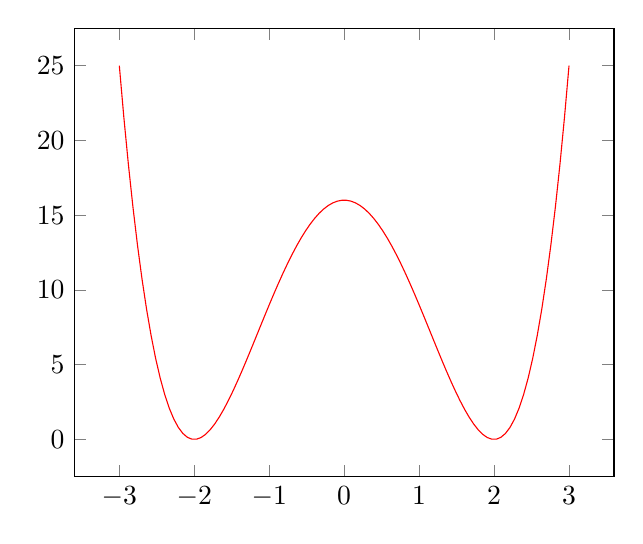
\begin{tikzpicture}
  \begin{axis}
    \addplot[color=red,domain=-3:3,samples=100]{x^4-8*x^2+16};
  \end{axis}
\end{tikzpicture}
\end{center}

\subsection{Globální (absolutní) extrémy}
\begin{enumerate}
  \item Definiční obor (může být zadán na intervalu)
  \item Derivace
  \item Nulové body derivace $f'(x)=0$
    \begin{enumerate}[label=(\alph*)]
      \item vypočítat
      \item vyjde konkrétní výsledek
      \item musí být v interavalu D(f)
    \end{enumerate}
  \item K nul. bodům D(f) přidáme hodnotu z $f'(x)=0$
  \item Do funkce f(x) zadáváme hodnoty x z nul. bodů
\end{enumerate}
\begin{equation}
  f(x)=\sqrt{2+x}+\sqrt{6-x}
\end{equation}
\hrule
\begin{align*}
  f'(x)&=\frac{\sqrt{6-x}-\sqrt{2+x}}{2*\sqrt{2+x}*\sqrt{6-x}}=0\\
       &=\sqrt{6-x}-\sqrt{2+x}=0\\
       x&=2\in\langle-2;6\rangle
\end{align*}
\begin{center}
\begin{tikzpicture}
  \begin{axis}
    \addplot[color=red,domain=-10:10,samples=100]{sqrt(2+x)+sqrt(6-x)};
  \end{axis}
\end{tikzpicture}
\end{center}

\subsection{Konvexita, konkávita}
\begin{enumerate}
  \item Definiční obor
  \item 1. derivace a 2. derivace
  \item Nulové body
    \begin{itemize}
      \item podezřelé z inflexe (mění se zde znaménko)
      \item zkontrolovat, zda leží v D(f)
    \end{itemize}
  \item Znaménko nulových bodů
    \begin{itemize}
      \item $\cup$ konvexní (+)
      \item $\cap$ konkávní (-)
    \end{itemize}
  \item Interval konvexity, konkávity
  \item Inflexe - inflexní body
    \begin{itemize}
      \item změna konvexity, konkávity
      \item definovaná, spojitá v bodě
      \item $I_1[x_1;y_1]$
    \end{itemize}

\end{enumerate}

